Translation, as we have seen in Section \ref{sc:fgt}, is forming the local expansion at a target box by combining the plane-wave expansions of all source boxes in its interaction list.  The cost of the direct scheme (\ref{e:w2l}) is $\bigO(K^3 p^3 |B|)$. The sweeping algorithm introduced in \cite{greengard98} and extended to multidimensions in \cite{fggt} brings down the complexity to $\bigO(3dp^d |B|)$ in $d$ dimensions. 

%Infact, we believe the following to be true. 
%\begin{conj}
%{\em If $|B| = n_b^3$, then the optimal cost of translation is $\bigO(3 d p^d)$ and the sweeping algorithm of %\cite{greengard98} achieves it.}
%\end{conj}

In most practical applications, unlike the uniform case, not all boxes exist. Predominantly, there are two kinds of non-empty box distributions:
%
\begin{itemize}
 \item Volume distribution, in which, each source box on an average has $\bigO(K^3)$ target boxes in its interaction list. The uniform distribution is an example of this class. They also arise from highly nonuniform volumetric distribution of sources resulting in zero-boxes wherever there are no sources within them. 
 
 \item Surface distribution, in which, each source box on an average has $\bigO(K^2)$ target boxes in its interaction list. These arise when the sources reside on two-dimensional manifolds (eg., a sphere) embedded in the volume. 
\end{itemize}
%   
% 

%\begin{prob}
%{\em Given a regular grid of size $1/n_b$ in the unit cube with $|B|$ non-zero boxes in it, find the optimal traversal path so that the cost of translation is minimized.
%}
%\end{prob}
%

Suppose the unit cube $[0, 1]^3$ is partitioned into $n_b^3$ regular boxes and $|B|$ of them are non-empty. There are two main drawbacks to the sweeping algorithm. First, a naive implementation stores data in all the $n_b^3$ boxes. This could be detrimental both for the volume and the surface distributions as, potentially, $|B| <\!< n_b^3$. Second, its performance is worse than the direct scheme for surface distributions. For example, consider the case where the sources reside on the sphere. The sweeping algorithm generates extra non-empty boxes around the initial spherical layer of boxes increasing their total number from $|B|$ to $\bigO(K^3 |B|)$. Thereby, the overall cost of sweeping algorithm is $\bigO(9 p^3 K^3 |B|)$. The direct scheme, on the other hand, requires $\bigO(p^3 K^2 |B|)$ because each source box has only $\bigO(K^2)$ target boxes in its interaction list. 

In this section, we propose two algorithms, one for volume and the other for surface distributions, that achieve optimal complexity and have minimal storage requirements. Given any arbitrary source distribution, it could be hard to distinguish which category the resulting non-empty box distribution falls into. We present a computationally inexpensive method to compute the cost of both algorithms {\em apriori} and pick the optimal of the two. 


%We propose a new algorithm for accelerating the plane-wave
%translations, which only needs $\mathcal{O}(|B|^\frac{d-1}{d})$ storage instead
%of $\mathcal{O}(|B|)$ storage as required by the sweeping algorithm from
%\cite{fggt}. For cases where direct computation is more efficient compared to the sweeping
%algorithm, for example when the sources are distributed on the surface of a sphere, we propose
%a new method to {\em a priori} estimate the best way to traverse space. We use the direct scheme if the estimated cost of the direct scheme is lower than that of the sweep. The method for estimating the cost of the most efficient direct scheme is described in Section \ref{sec:mst}.

% NOT CORRECT ...
% In addition, the algorithm is work optimal for distributions with \ul{distribution density} less than $60\%$ (for $d=3$).

\subsection{Modified sweeping algorithm for volume distributions} 
\label{sec:sweep}

Instead of sweeping along each dimension one-by-one as proposed 
in \cite{fggt}, our algorithm visits each box only once and computes the full plane-wave
translation based on its neighbours which have already been visited. The
plane-wave expansions at a box $B_i$ can be represented as a combination of the
plane-wave expansions of its $2^{d} -1$ neighbours, along with corrections for
$2^d$ boxes. We start with direct computation of the outermost layer, and then propagate it inwards, layer by layer, as illustrated in Figure \ref{fig:sweep}. This results in an overall complexity of the sweep algorithm as $\mathcal{O}((2^{d+1} -1)p^d|B|)$. The constant in the
complexity for this step increases from $3d\rightarrow2^{d+1} - 1$, which is
from $6\rightarrow7$ for $d=2$ and from $9\rightarrow15$ for $d=3$. 

The algorithm is illustrated in Figure \ref{fig:w2l}. The steps involved in the
algorithm are as follows, 
\begin{enumerate}    
  \item First compute the local expansions at the outermost layer of the FGT
    boxes. Full computation ($K^dp^d$) is only required for the first box, as
    the local expansions for the other boxes can be computed by adding and
    subtracting layers from the expansions of the already computed boxes. 
  
  \item We propagate the local expansions from this initial layer to subsequent
    layers. Consider the case shown in Figure \ref{fig:w2l} where we need to
    compute the local expansion of the Green box ( $B(i+1,j+1)$), given the
    local expansions of the adjacent boxes (in Orange).  
  
  \item The local expansion $v_k^{B(i+1, j+1)}$ can be written in terms for the
    local expansions of the $2^d -1$ neighbours $B(i,j), B(i+1,j)$ and
    $B(i,j+1)$, along with corrections terms from the $2^d$ corners.
    These are marked in Figure \ref{fig:w2l} assuming $K=3, n=1$. 
    The local expansion can therefore be computed as,
    \begin{eqnarray*} 
    % v_k^{i+1,j+1} &=& \sum_{\eta_{i,j} = 0,1} (-1)^{1 + d + |\eta|_1} e^{i\lambda k\cdot\eta} v_k^{i+\eta_i, j+\eta_j} \\
    v_k^x &=& \sum_{\eta \in \mathcal{N}(x)} (-1)^{1 + d + |\eta|_1} e^{i\lambda k\cdot\eta} v_k^{x+\eta} \\
    % & +& \sum_{\eta_{i,j}= 0,1} (-1)^{1 + d + |\eta|_1} e^{iz_k\eta ns/\sqrt{\delta}} w_k^{i+\eta_i, j+\eta_j}.
    & +& \sum_{\chi \in \mathcal{C}(x)} (-1)^{1 + d + |\chi|_1} e^{i\lambda k\cdot\chi} w_k^{x+\chi}.
    \end{eqnarray*}
    where $\mathcal{C}(\cdot)$ assigns the sign to the contribution of the specific neighbour or corner. Specifically, it is 
    \[
      \mathcal{C}(x) = (-1)^{1+d+|x|_1}
    \]
    
 %   e^{iz_k s/\sqrt{\delta}} v_k^{i+1,j} + e^{iz_k s/\sqrt{\delta}} v_k^{i,j+1} - e^{iz_k s/\sqrt{\delta}} v_k^{i,j} - e^{iz_k ns/\sqrt{\delta}} w_k^{i+n+1,j+n+1} + e^{-iz_k ns/\sqrt{\delta}} w_k^{i-n,j-n}
  
  \item The propagation can then be used to propagate to the remaining boxes in
    the new propagation layer. At any given stage only the values of the
    propagation layer needs to be stored. The values at any box with zero
    coefficient can therefore be ignored and need not be stored.

\end{enumerate}


\begin{figure}
\centering
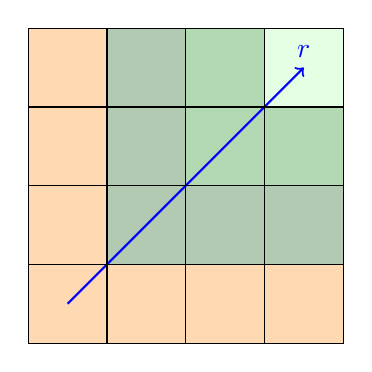
\begin{tikzpicture}[scale=0.5]
	
	\draw[fill=orange!30] (0,0) rectangle +(8,2);
	\draw[fill=orange!30] (0,2) rectangle +(2,6);

	\draw[fill=green!30!black!30] (2,2) rectangle +(6,2);
	\draw[fill=green!30!black!30] (2,4) rectangle +(2,4);
	
	\draw[fill=green!50!black!30] (4,4) rectangle +(4,2);
	\draw[fill=green!50!black!30] (4,6) rectangle +(2,2);
	
	\draw[fill=green!10] (6,6) rectangle +(2,2);
	
	% arrows ...
	\draw[blue, thick, ->] (1,1) -- (7,7) node[above] {$r$}; 
												
	% the grid ...
	\draw[step=2cm] (0,0) grid (8,8);	
	
\end{tikzpicture}
\caption{\small The outermost layer is shown in orange, for which the local expansions are computed directly. The other layers (in green) are computed by propagation. The direction of propagation ($r$) is shown using the arrow and by the shade of the layers, lighter being later in time.
}
\label{fig:sweep}
\end{figure}

\begin{figure}
\centering
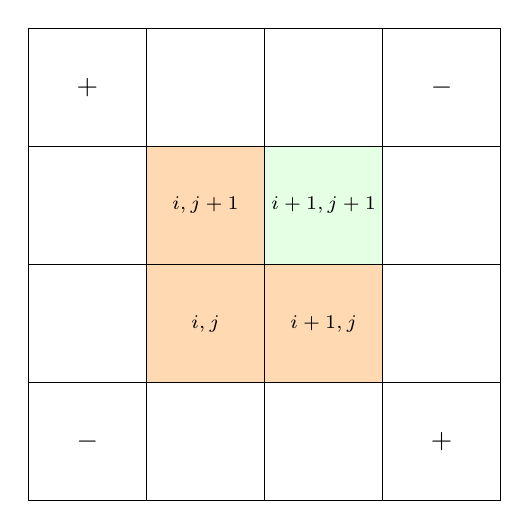
\begin{tikzpicture}[scale=0.75]
	
	\draw[fill=orange!30] (2,2) rectangle +(4,2);
	\draw[fill=orange!30] (2,2) rectangle +(2,4);
	
	\draw[fill=green!10] (4,4) rectangle +(2,2);		
	% the grid ...
	\draw[step=2cm] (0,0) grid (8,8);	
	
	\draw (3,3) node {\scriptsize{$i, j$}};
	\draw (5,3) node {\scriptsize{$i+1, j$}};
	\draw (3,5) node {\scriptsize{$i, j+1$}};
	\draw (5,5) node {\scriptsize{$i+1, j+1$}};
	
	\draw (1,1) node {$-$};
	\draw (7,7) node {$-$};
	\draw (1,7) node {$+$};
	\draw (7,1) node {$+$};
			
\end{tikzpicture}
\caption{\small The propagation of the local expansions using neighbors. 
}
\label{fig:w2l}
\end{figure}

\subsection{Modified sweeping algorithm for surface distributions} 
\label{sec:mst}
For surface distributions, the algorithm introduced in the previous section generates large number of additional non-empty boxes and consequently it becomes computationally more expensive than the direct scheme. We introduce a new approach here that does not generate any extra non-empty boxes and performs better than the direct scheme. 

The main idea, however, is similar: once a local expansion is formed at a particular box, we use this information to minimize the translation cost at a subsequently visited box. At the first box $B_1$ we form the local expansion directly with $\displaystyle \mathcal{O}\left(\,|\mathcal{I} [B_1]| \, p^3\right)$ work, where $|\cdot|$ is the size of the set. For subsequent boxes, we only need to add/sustract the plane-wave expansions of the boxes that are not present in both the interaction lists of the current box and that of the previously visited box. The problem is therefore to determine the optimal traversal such that the overall cost is reduced.

\begin{prob}[Optimal Traversal] {\em Find an ordering $\{ B_1, B_2, \ldots, B_{|B|}\}$ so that 
%
\beq |\mathcal{I}[B_1]| + \sum_{j=1}^{|B|-1} |\mathcal{I}(B_j)\cup\mathcal{I}(B_{j+1}) - \mathcal{I}(B_j)\cap\mathcal{I}(B_{j+1})| \eeq
%
is minimized.}
\end{prob}

There are many ways to find the optimal traversal path. We take a graph theory approach by reducing optimal traversal problem to finding the minimum spanning tree of a graph. 

\begin{prob}[MST] {\em Construct a weighted graph $G = (V, E)$ with the non-empty FGT boxes as its vertices. 
An edge is introduced between vertices $v_i$ and $v_j$ if and only if $B_i \in \mathcal{I}[B_j]$. The weight of an edge between boxes $B_i$ and $B_j$ is given by
%
\beq w_{ij} = |\mathcal{I}(B_i)\cup\mathcal{I}(B_{j}) - \mathcal{I}(B_j)\cap\mathcal{I}(B_{j})|. \eeq
%
Introduce an additional vertex $v*$ which connects to every vertex $v_i$ in the graph by an edge whose weight is equal to $|\mathcal{I}[B_i]|$. Find the minimum spanning tree of $G$.}
\end{prob}

The vertex $v*$ encodes the cost of the direct computation at the first box. 

We compute the minimum spanning tree of this graph using Kruskal's algorithm \cite{kruskal56} whose complexity is $\mathcal{O}(|E| \log |V|)$, which in our case becomes $\mathcal{O}(K^2 |B| \log |B|)$ because $|E| = K^2 |B|$ and $|V| = |B|$.
 
%Each of the remaining vertices (FGT boxes) are connected to a maximum of $26$ other vertices (corresponding to the immediate non-zero neighbors of the box). 

The total cost of the tree is used to determine whether to use the direct approach or to use the sweeping or the propagation scheme described in Section \ref{sec:sweep}. The edges of the tree gives us the optimal traversal to compute the plane-wave translations.
\begin{table}
\centering
\begin{tabular}{cccc} \hline
        $|B|$  &  direct & MST & ratio \\ \hline       
        \multicolumn{4}{c}{}  \\
        \multicolumn{4}{c}{ {\small $K =  9 \quad (\epsilon = 10^{-6})$}}  \\
        \multicolumn{4}{c}{}  \\
         1K & & &  \\  
        100K & & &  \\  
       1000K & & &  \\  
       \multicolumn{4}{c}{}  \\
       \multicolumn{4}{c}{ {\small $K =  13 \quad (\epsilon = 10^{-12})$}}  \\
       \multicolumn{4}{c}{}  \\
             1K & & &  \\  
        100K & & &  \\  
       1000K & & &  \\  
\hline
\end{tabular}
\end{table}


\begin{figure}
\centering 	
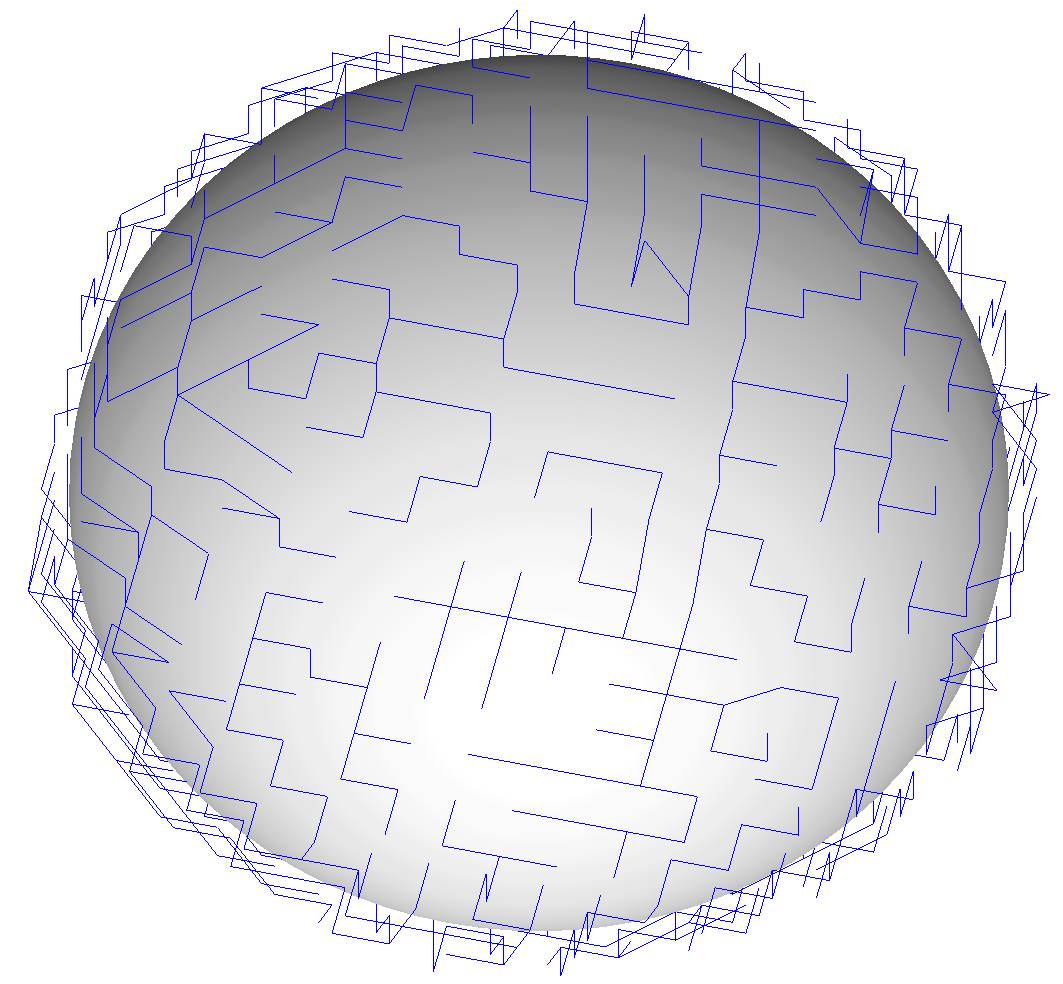
\includegraphics[width=0.4\textwidth]{figs/sphere_mst}
\caption{The optimal traversal path for a spherical shell distribution, shown here superimposed on a sphere. The nodes of the graph are the centers of the boxes $B_i$.}
\end{figure}

